This section presents our results. The first sub-section contains summary statistics regarding the variability of six key covariates pre- and post- adjustment to address measurement error. The second sub-section contains covariate balance diagnostics. The third sub-section contains our primary ETC results, presenting our estimates of the treatment effect and a series of sensitivity analyses. The final sub-section contains our analysis of covariate importance and investigation into treatment effect heterogeneity.

\subsection{Covariate adjustment}

We first examine the effects of our covariate adjustments on the variance of our pre-treatment outcomes and pre-treatment unemployment rates among the expansion states. We most heavily prioritize balancing these covariates, but they are also among the least precisely estimated (all of our other covariates average over three years of data, rather than just one). Table~\ref{tab:adjust1} displays the variance of each covariate on the unadjusted and adjusted datasets. We see that both the homogeneous and heterogeneous adjustment procedures reduce the variability in the data by comparable amounts. Intuitively, the adjustment to address measurement error reduces the likelihood that our balancing weights will over-fit to noise in the data. These results are consistent across most of our other covariates.

\begin{table}[ht]
\caption{Sample variance on unadjusted and adjusted datasets, expansion states}
\label{tab:adjust1}
\begin{tabular}{lrrr}
  \hline
Variable & No adjustment & Heterogeneous & Homogeneous \\ 
  \hline
Uninsured Pct 2011 & 8.35 & 8.04 & 8.05 \\ 
  Uninsured Pct 2012 & 8.20 & 7.89 & 7.90 \\ 
  Uninsured Pct 2013 & 8.09 & 7.78 & 7.79 \\ 
  Unemployed Pct 2011 & 3.66 & 3.25 & 3.27 \\ 
  Unemployed Pct 2012 & 3.72 & 3.38 & 3.38 \\ 
  Unemployed Pct 2013 & 3.20 & 2.88 & 2.87 \\ 
   \hline
\end{tabular}
\end{table}

\subsection{Covariate balance}

Figure~\ref{fig:loveplotc1} displays the reduction of imbalances using our H-SBW weights. This plot only displays covariates with greater than one percentage point difference between the targeted mean in the expansion region and the mean values in the non-expansion region prior to weighting, and the reweighted treatment values use our preferred covariate adjustment $\hat{\eta}_1(W_{sc})$. Before applying our weights, we see that there are substantial imbalances in the Republican governance indicators, as well as pre-treatment uninsurance and unemployment rates. Our weights reduce these differences; however, some remain, particularly among the Republican governance indicators. A complete balance table is available in Appendix D, Table~\ref{tab:baltab1}. 

\begin{figure}[H]
\begin{center}
    \caption{Balance plot, primary dataset}
    \label{fig:loveplotc1}
    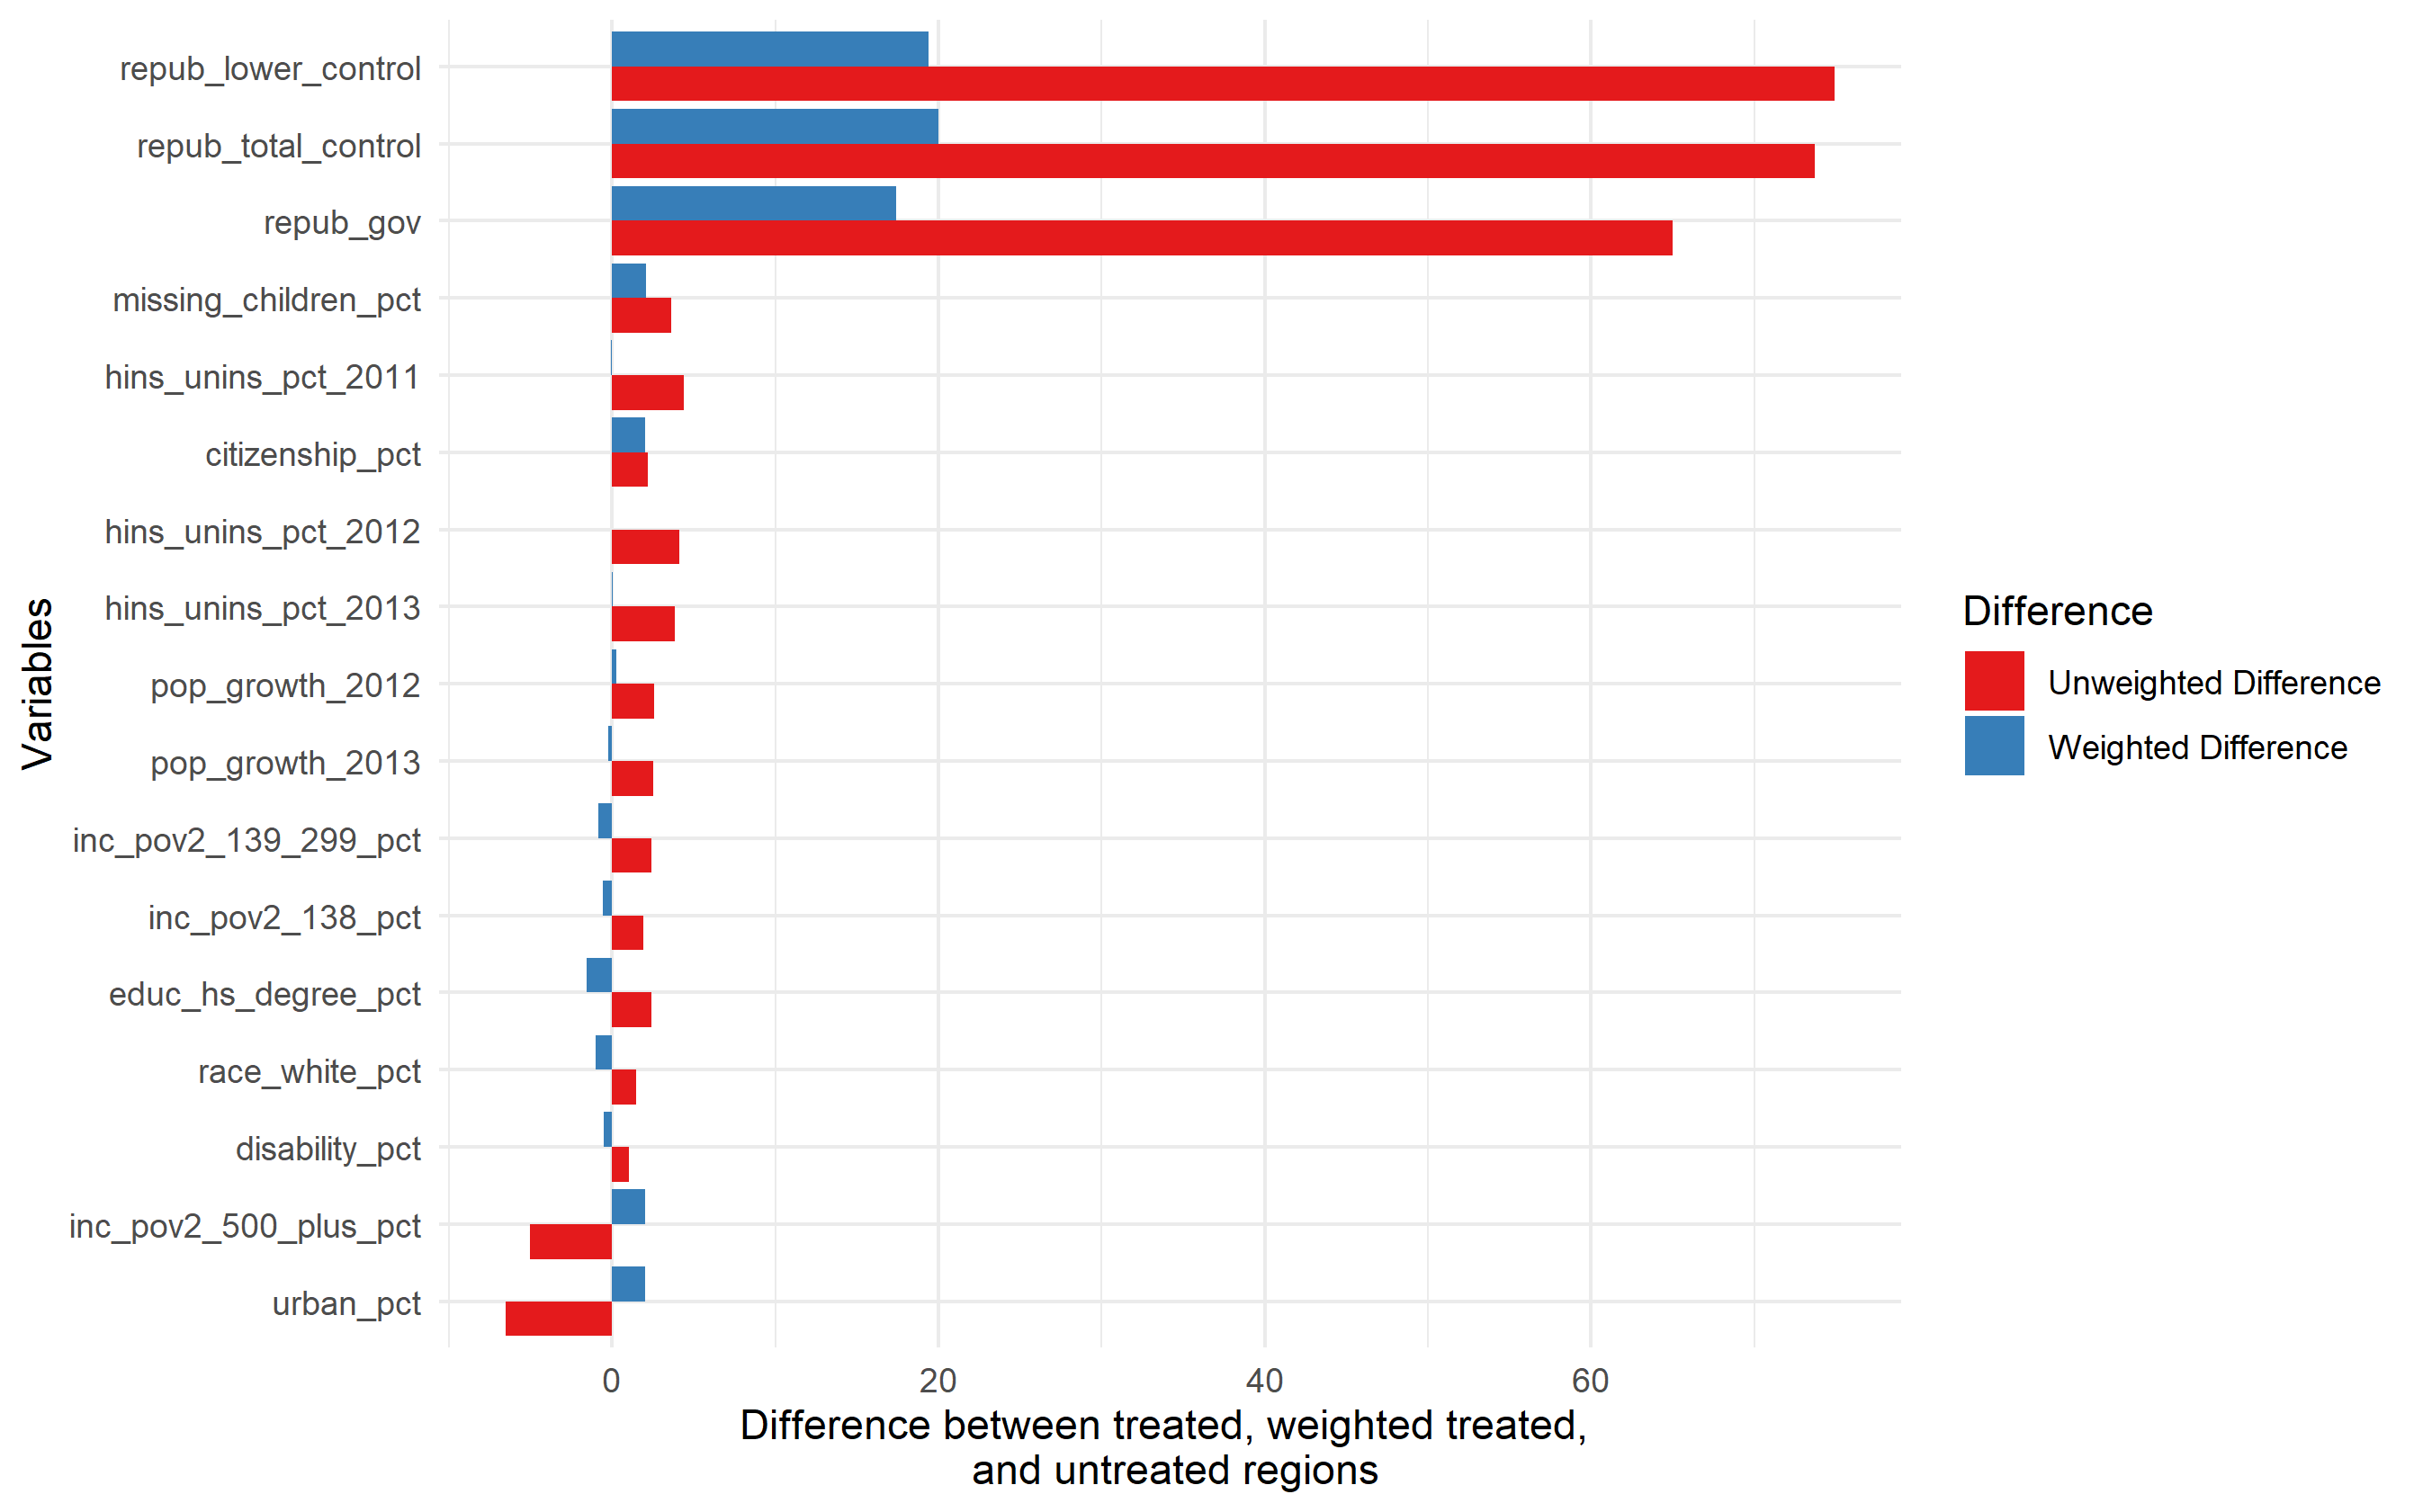
\includegraphics[scale=0.6]{01_Plots/balance-plot-etuc1.png}
\end{center}
\end{figure}

We also compare the H-SBW estimator to the SBW estimates in Figure~\ref{fig:sbwvhsbw1}. We see that H-SBW more evenly distributes the weights across states relative to SBW, particularly by reducing the amount of weight given to CPUMAs in Ohio. 

\begin{figure}[H]
\begin{center}
    \caption{H-SBW versus SBW, weights summed by state, primary dataset}
    \label{fig:sbwvhsbw1}
    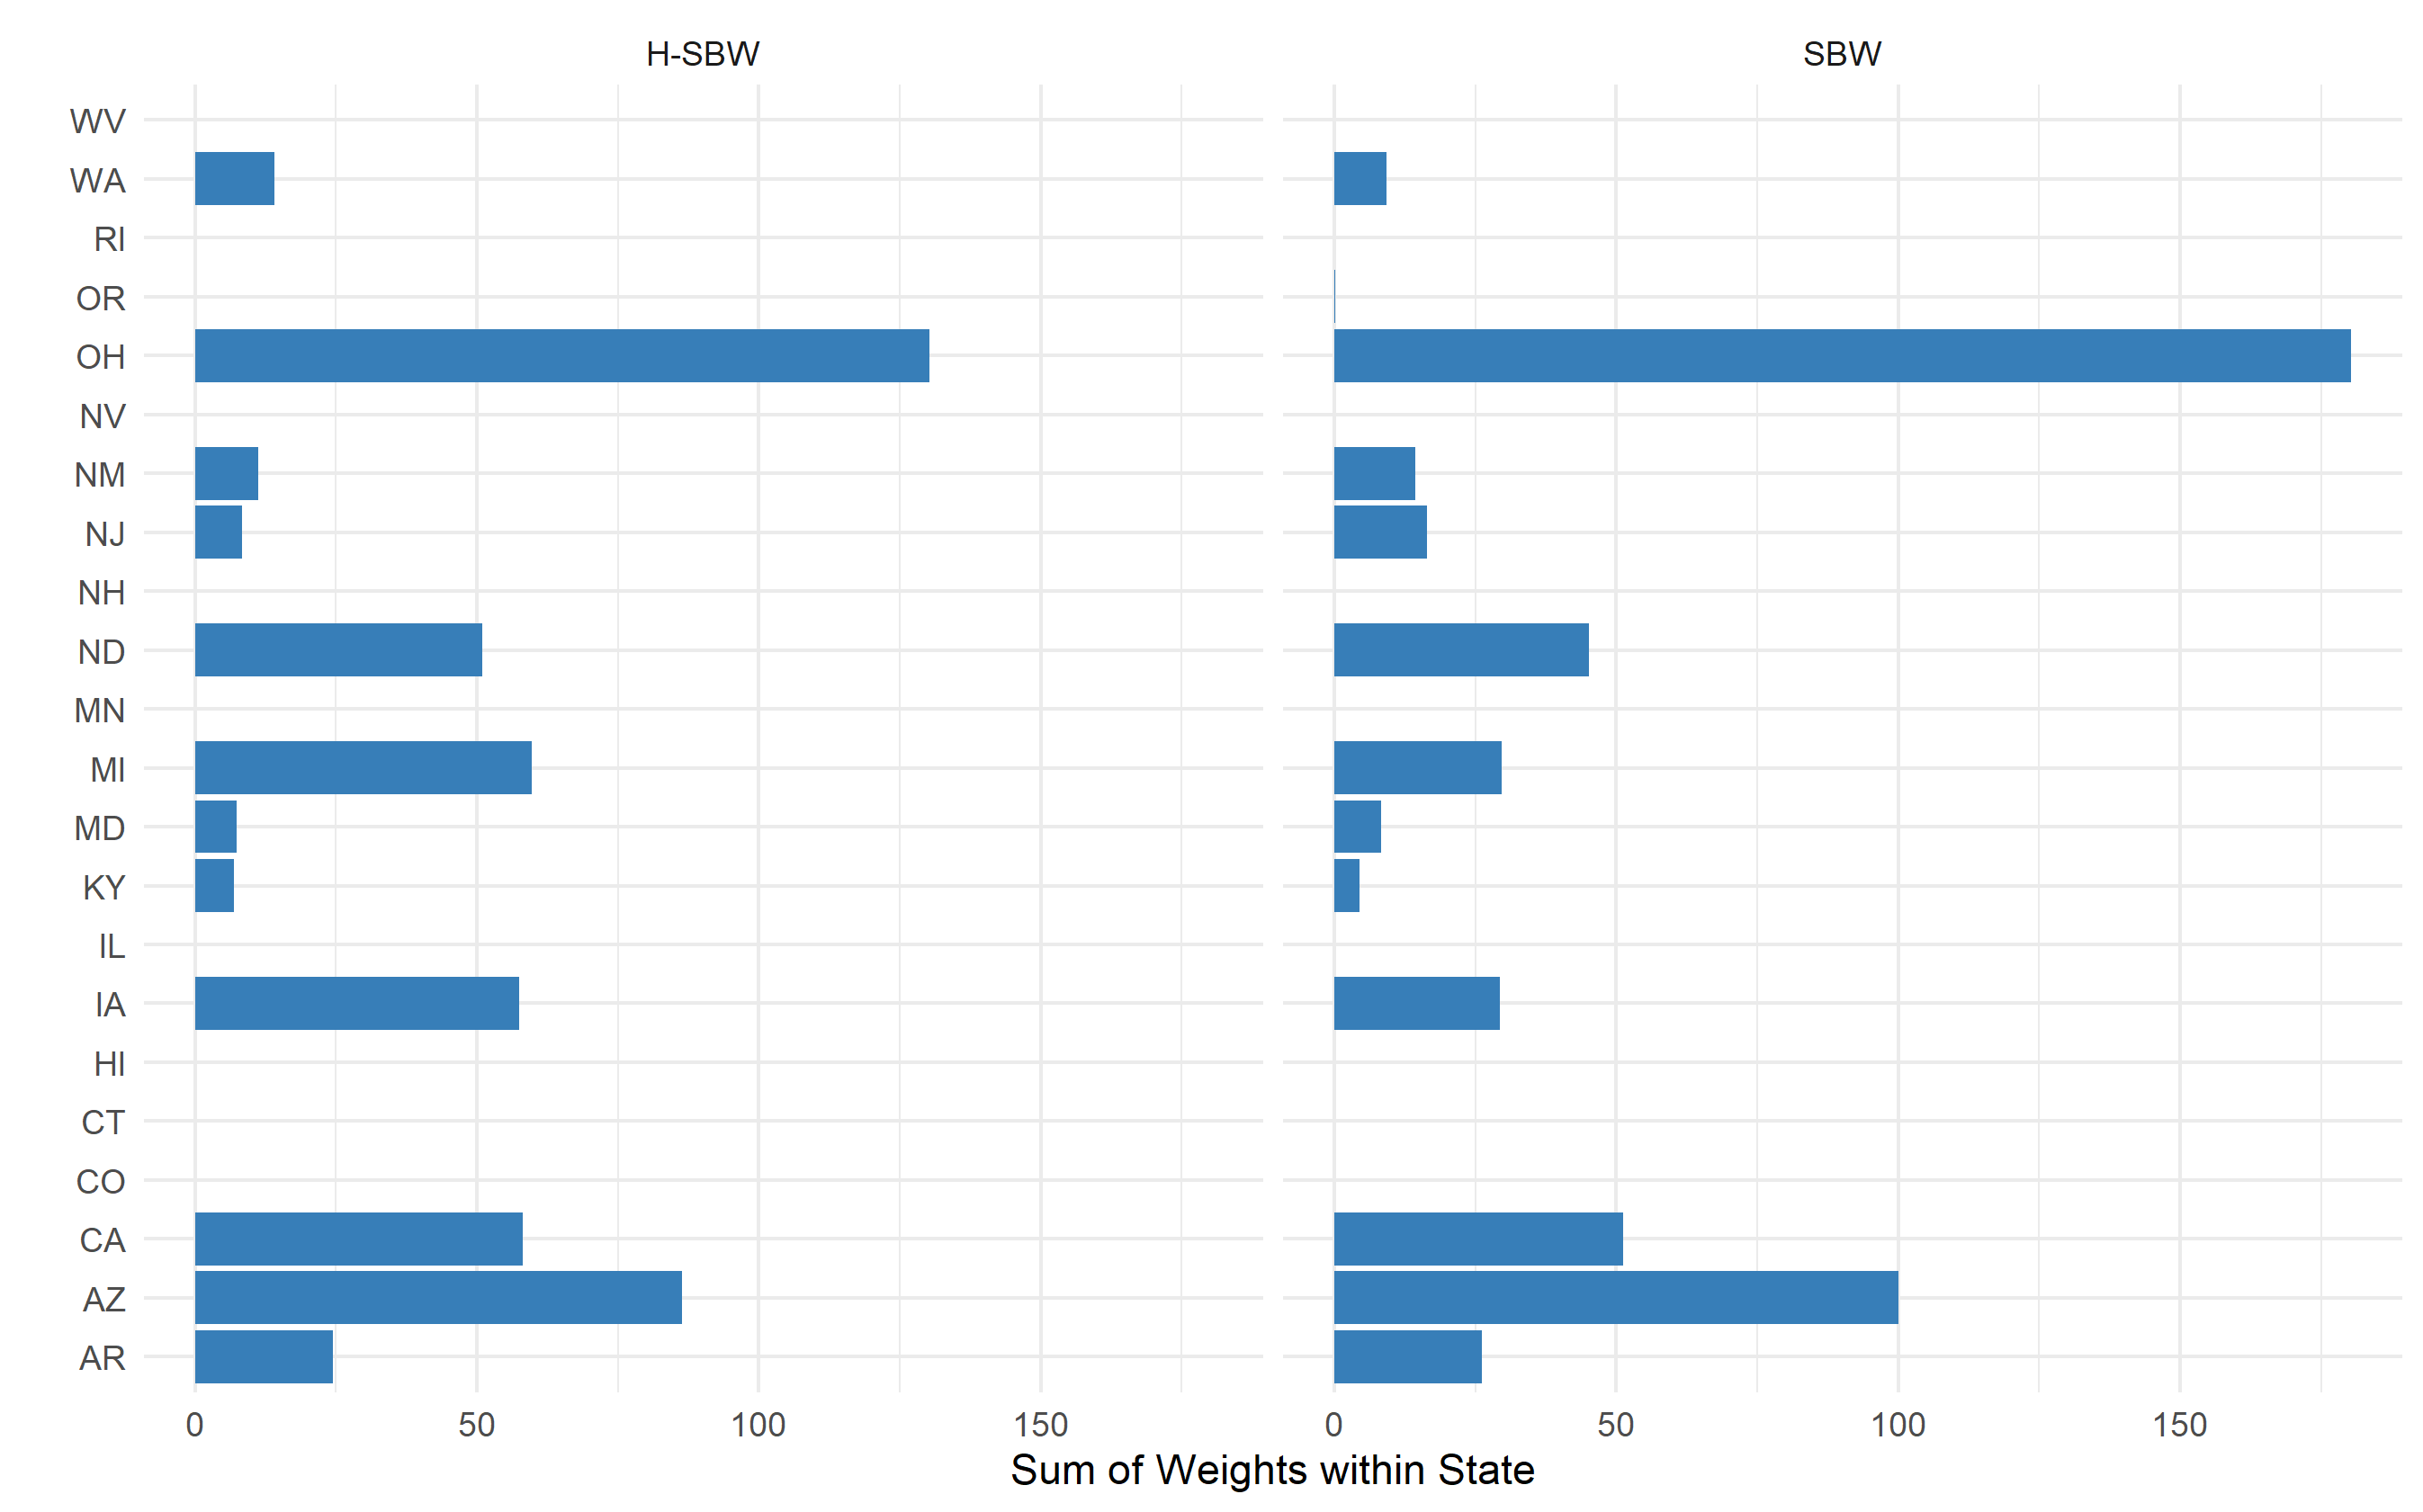
\includegraphics[scale=0.6]{01_Plots/weights-by-state-sbw-hsbw-c1.png}
\end{center}
\end{figure}

We then use ridge-regression augmentation to extrapolate from the data in order to reduce all imbalances within 0.5 percentage points. Figure~\ref{fig:statewghts} shows the total weights summed across states for two estimators: H-SBW and BC-HSBW. This figure sums the negative weights separately from the positive weights to show the extent of the extrapolation. We see that BC-HSBW extrapolates somewhat heavily in order to achieve the desired level of balance, particularly for CPUMAs in California. 

\begin{figure}[H]
\begin{center}
    \caption{H-SBW versus BC-HSBW, weights summed by state, primary dataset}
    \label{fig:statewghts}
    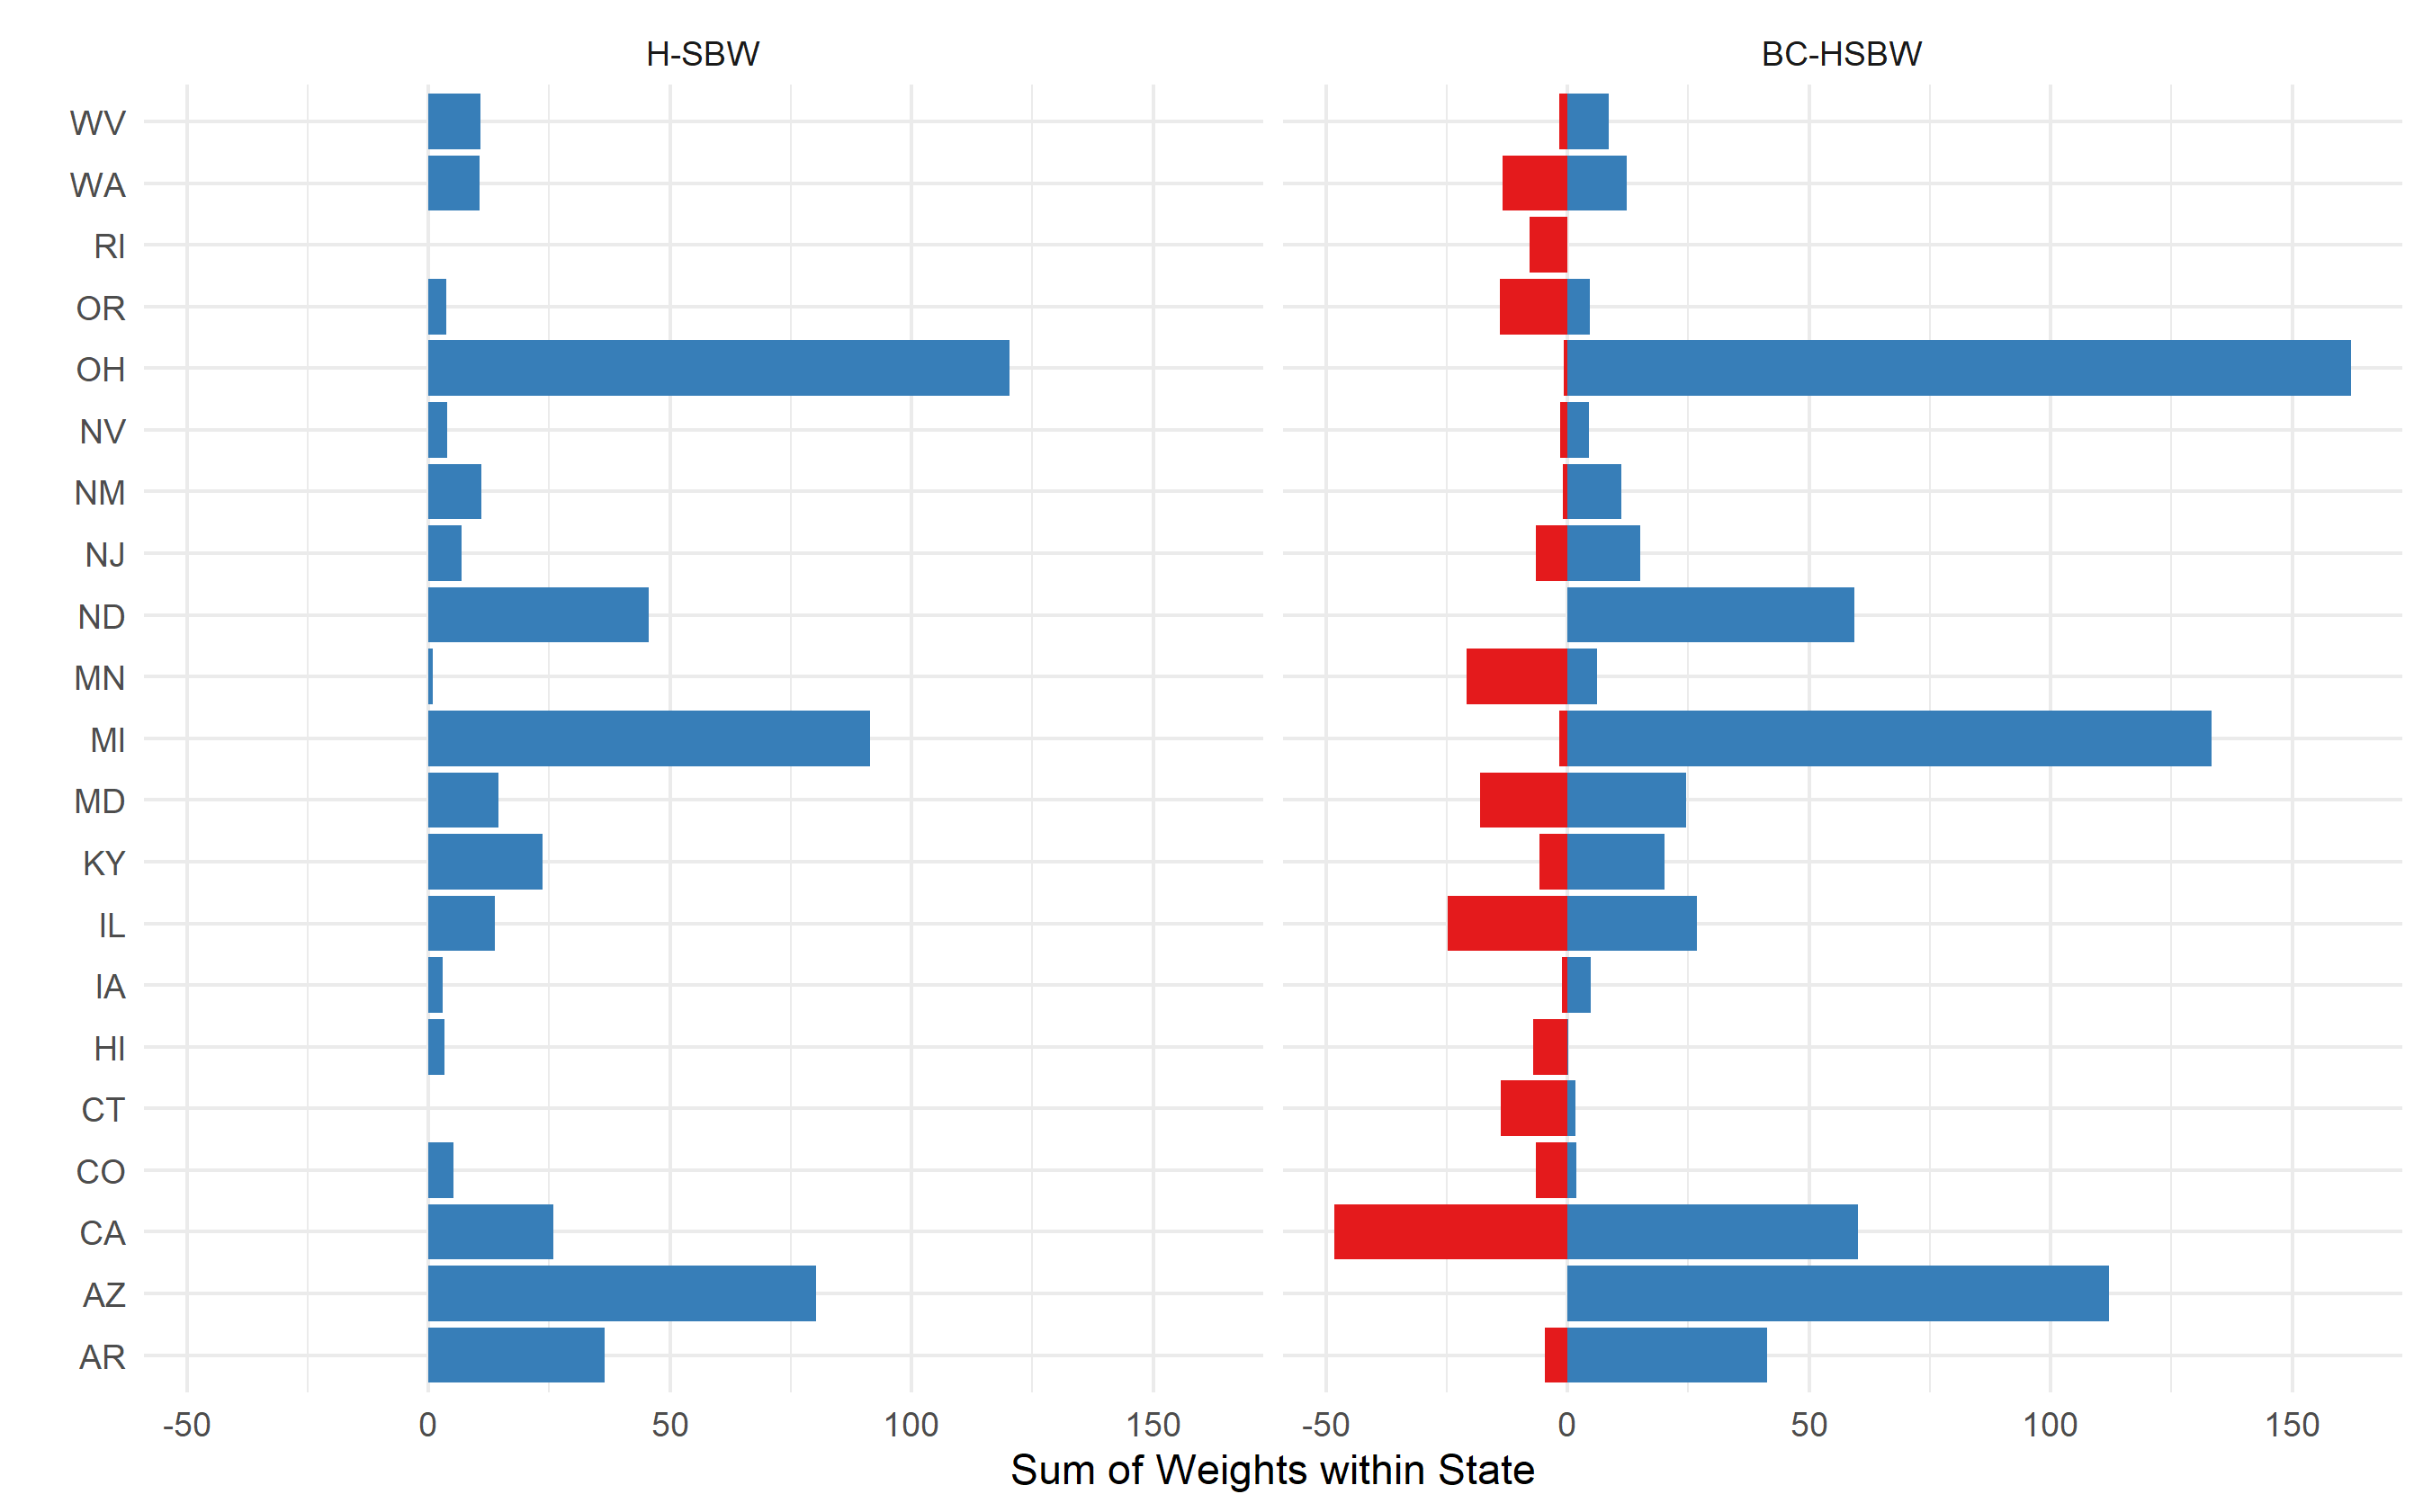
\includegraphics[scale=0.6]{01_Plots/weights-by-state-hsbw-c1.png}
\end{center}
\end{figure}

Finally, we wish to see whether the weights generated using the unadjusted data balance the adjusted covariates. While this balance measure does not reflect the ``true'' imbalances, this comparison does give some indication of whether the unadjusted weights are overfitting to noisy covariate measurements. Table~\ref{tab:balcomp} compares the imbalances among our pre-treatment outcomes and uninsurance rates using H-SBW weights generated on our unadjusted dataset applied to the adjusted (homogeneous) dataset. The ``Unweighted Difference'' column represents the raw difference in means, while the ``Weighted Diff'' column reflects the weighted difference that we calculate on the unadjusted dataset. The ``Homogeneous Diff'' column displays the weighted imbalance when applying the H-SBW weights to the dataset using the homogeneous adjustment, and likewise for ``Heterogeneous Diff.'' We see that the weighted pre-treatment outcomes are approximately one percentage point lower than we desired in the two years prior to treatment using the heterogeneous adjustment, and -0.2 percentage points lower (on average) using the homogeneous adjustment. Given the high degree of correlation between pre-treatment outcomes, we may expect the estimator of $\psi^1$ trained on the unadjusted data to have some downward bias.

\begin{table}[ht]
\caption{Balance comparison: unadjusted weights on adjusted data}
\label{tab:balcomp}
\begin{tabular}{lrrrr}
  \hline
Variables & Unweighted Diff & Weighted Diff (none) & Homogeneous Diff & Heterogeneous Diff\\ 
  \hline
Uninsured Pct 2011 & -3.09 & -0.05 & -0.11 & 0.92 \\ 
  Uninsured Pct 2012 & -2.99 & -0.05 & -0.21 & -1.06 \\ 
  Uninsured Pct 2013 & -3.00 & -0.05 & -0.38 & -0.93 
   \hline
\end{tabular}
\end{table}

\subsubsection{Model validation}

We compare the performance of our models by repeating the covariate adjustments and calculating our procedure on 2009-2011 ACS data to predict 2012 outcomes, and similarly for 2010-2012 data to predict 2013 outcomes for the treated states. Table~\ref{tab:pretxpred} see that the estimators trained on the covariate adjusted data have substantially better performance than the unadjusted data. Moreover, the estimators trained on the homogeneous adjustment seem to do slightly better than the ones that model the heterogeneity; we therefore prioritize presenting results on the homogeneous adjustment. We also find that SBW tends to have slightly lower bias than H-SBW. This is consistent with our theoretic results in Appendix A, which show that the bias should decrease with the square of the weights for fixed $X$. Despite these results, H-SBW may have lower variance (and possibly MSE) given our assumed dependencies in the model errors. We therefore do not use these results to prefer H-SBW or SBW. Finally, we see that the bias corrected estimators tend to perform worse in this application. This indicates that the extrapolation bias outweighs the cost of the covariate imbalances. While this does not necessarily imply this should hold for the model of $Y^1_T$, it does caution against these results. We see this as a function of our models as best reflecting an approximation: we expect in general that assuming the linear outcome models approximately holds on the support of the data where we have sufficient covariate overlap, but we these models may lead us astray when our weights extrapolate excessively from the data. The worst performing estimators are the bias-corrected estimators trained on the unadjusted data.

\begin{table}[ht]
\caption{Estimator pre-treatment outcome prediction error}
\label{tab:pretxpred}
\begin{tabular}{llrrr}
  \hline
Sigma estimate & Estimator & 2012 error & 2013 error & RMSE \\ 
  \hline
Homogeneous & SBW & -0.18 & -0.22 & 0.20 \\ 
  Homogeneous & H-SBW & -0.24 & -0.21 & 0.23 \\ 
  Heterogeneous & SBW & -0.25 & -0.30 & 0.27 \\ 
  Heterogeneous & H-SBW & -0.32 & -0.39 & 0.36 \\ 
  Homogeneous & BC-SBW & -0.42 & -0.35 & 0.39 \\ 
  Heterogeneous & BC-SBW & -0.45 & -0.39 & 0.42 \\ 
  None & SBW & -0.50 & -0.61 & 0.56 \\ 
  None & H-SBW & -0.52 & -0.61 & 0.57 \\ 
  Homogeneous & BC-HSBW & -0.53 & -0.62 & 0.58 \\ 
  Heterogeneous & BC-HSBW & -0.53 & -0.72 & 0.63 \\ 
  None & BC-SBW & -0.82 & -0.93 & 0.88 \\ 
  None & BC-HSBW & -0.93 & -0.99 & 0.96 \\ 
   \hline
\end{tabular}
\end{table}

Finally, we find a consistent negative bias across all of our estimators: that is, all of our models tend to under-predict the true uninsurance rate among the non-expansion states the subsequent year. If we believe that the sign of this bias will also afflict our estimates of $\bar{Y}^1$, then we should expect our treatment effect estimates to have downward bias (which would bias our estimates away from zero). That is, the true treatment effect may be smaller (closer to zero) in absolute magnitude than the estimated treatment effect. If we believe the bias will also have comparable magnitude, these results suggests that the true treatment effect will be approximately 0.2 to 0.5 percentage points closer to zero than the estimated effect.

\subsection{Primary Results}

Using H-SBW we estimate an effect of -2.33 (-3.49, -1.16) percentage points. The SBW results are almost identical with -2.35 (-3.65, -1.06) percentage points. Compared to the unadjusted data we see very similar estimates at -2.34 (-2.85, -1.82) percentage points for H-SBW and -2.39 (-2.95, -1.83) percentage points for SBW. We see that H-SBW reduces the confidence intervals relative to SBW. We also observe that using the adjusted covariate set appears to increases the width of the estimated confidence intervals. This increase in variability is expected because the adjustment procedure generally reduces the variability in the data, as we saw in Table~\ref{tab:adjust1}, thereby requiring that the balancing weights also increase in variability to achieve the desired level of balance. Importantly, this variance estimate conditions on the covariate adjustment, and does not take into account the randomness in this procedure, and may therefore understate the true uncertainty. When we recalculate the entire adjustment procedure, we find that the confidence intervals are of a comparable magnitude. The results are available in Appendix E.

When we add the bias-correction, the absolute magnitude of the point estimate decreases: we estimate -2.05 (-3.32, -0.79) percentage points for BC-HSBW and -2.00 (-2.98, -1.01) percentage points for BC-SBW. In contrast to the H-SBW and SBW estimators, we see that the confidence interval for BC-SBW is narrower than for BC-HSBW. Figure~\ref{fig:estimators} presents all of our estimates. All adjusted estimates were closer to zero than the unadjusted estimates, though the point estimates from the SBW and H-SBW were estimators were virtually identical. The heterogeneous adjustments were all closer to zero than the unadjusted estimates; results are available in Appendix E.

\begin{figure}[H]
\begin{center}
    \caption{Primary point estimates and confidence intervals}
    \label{fig:estimators}
    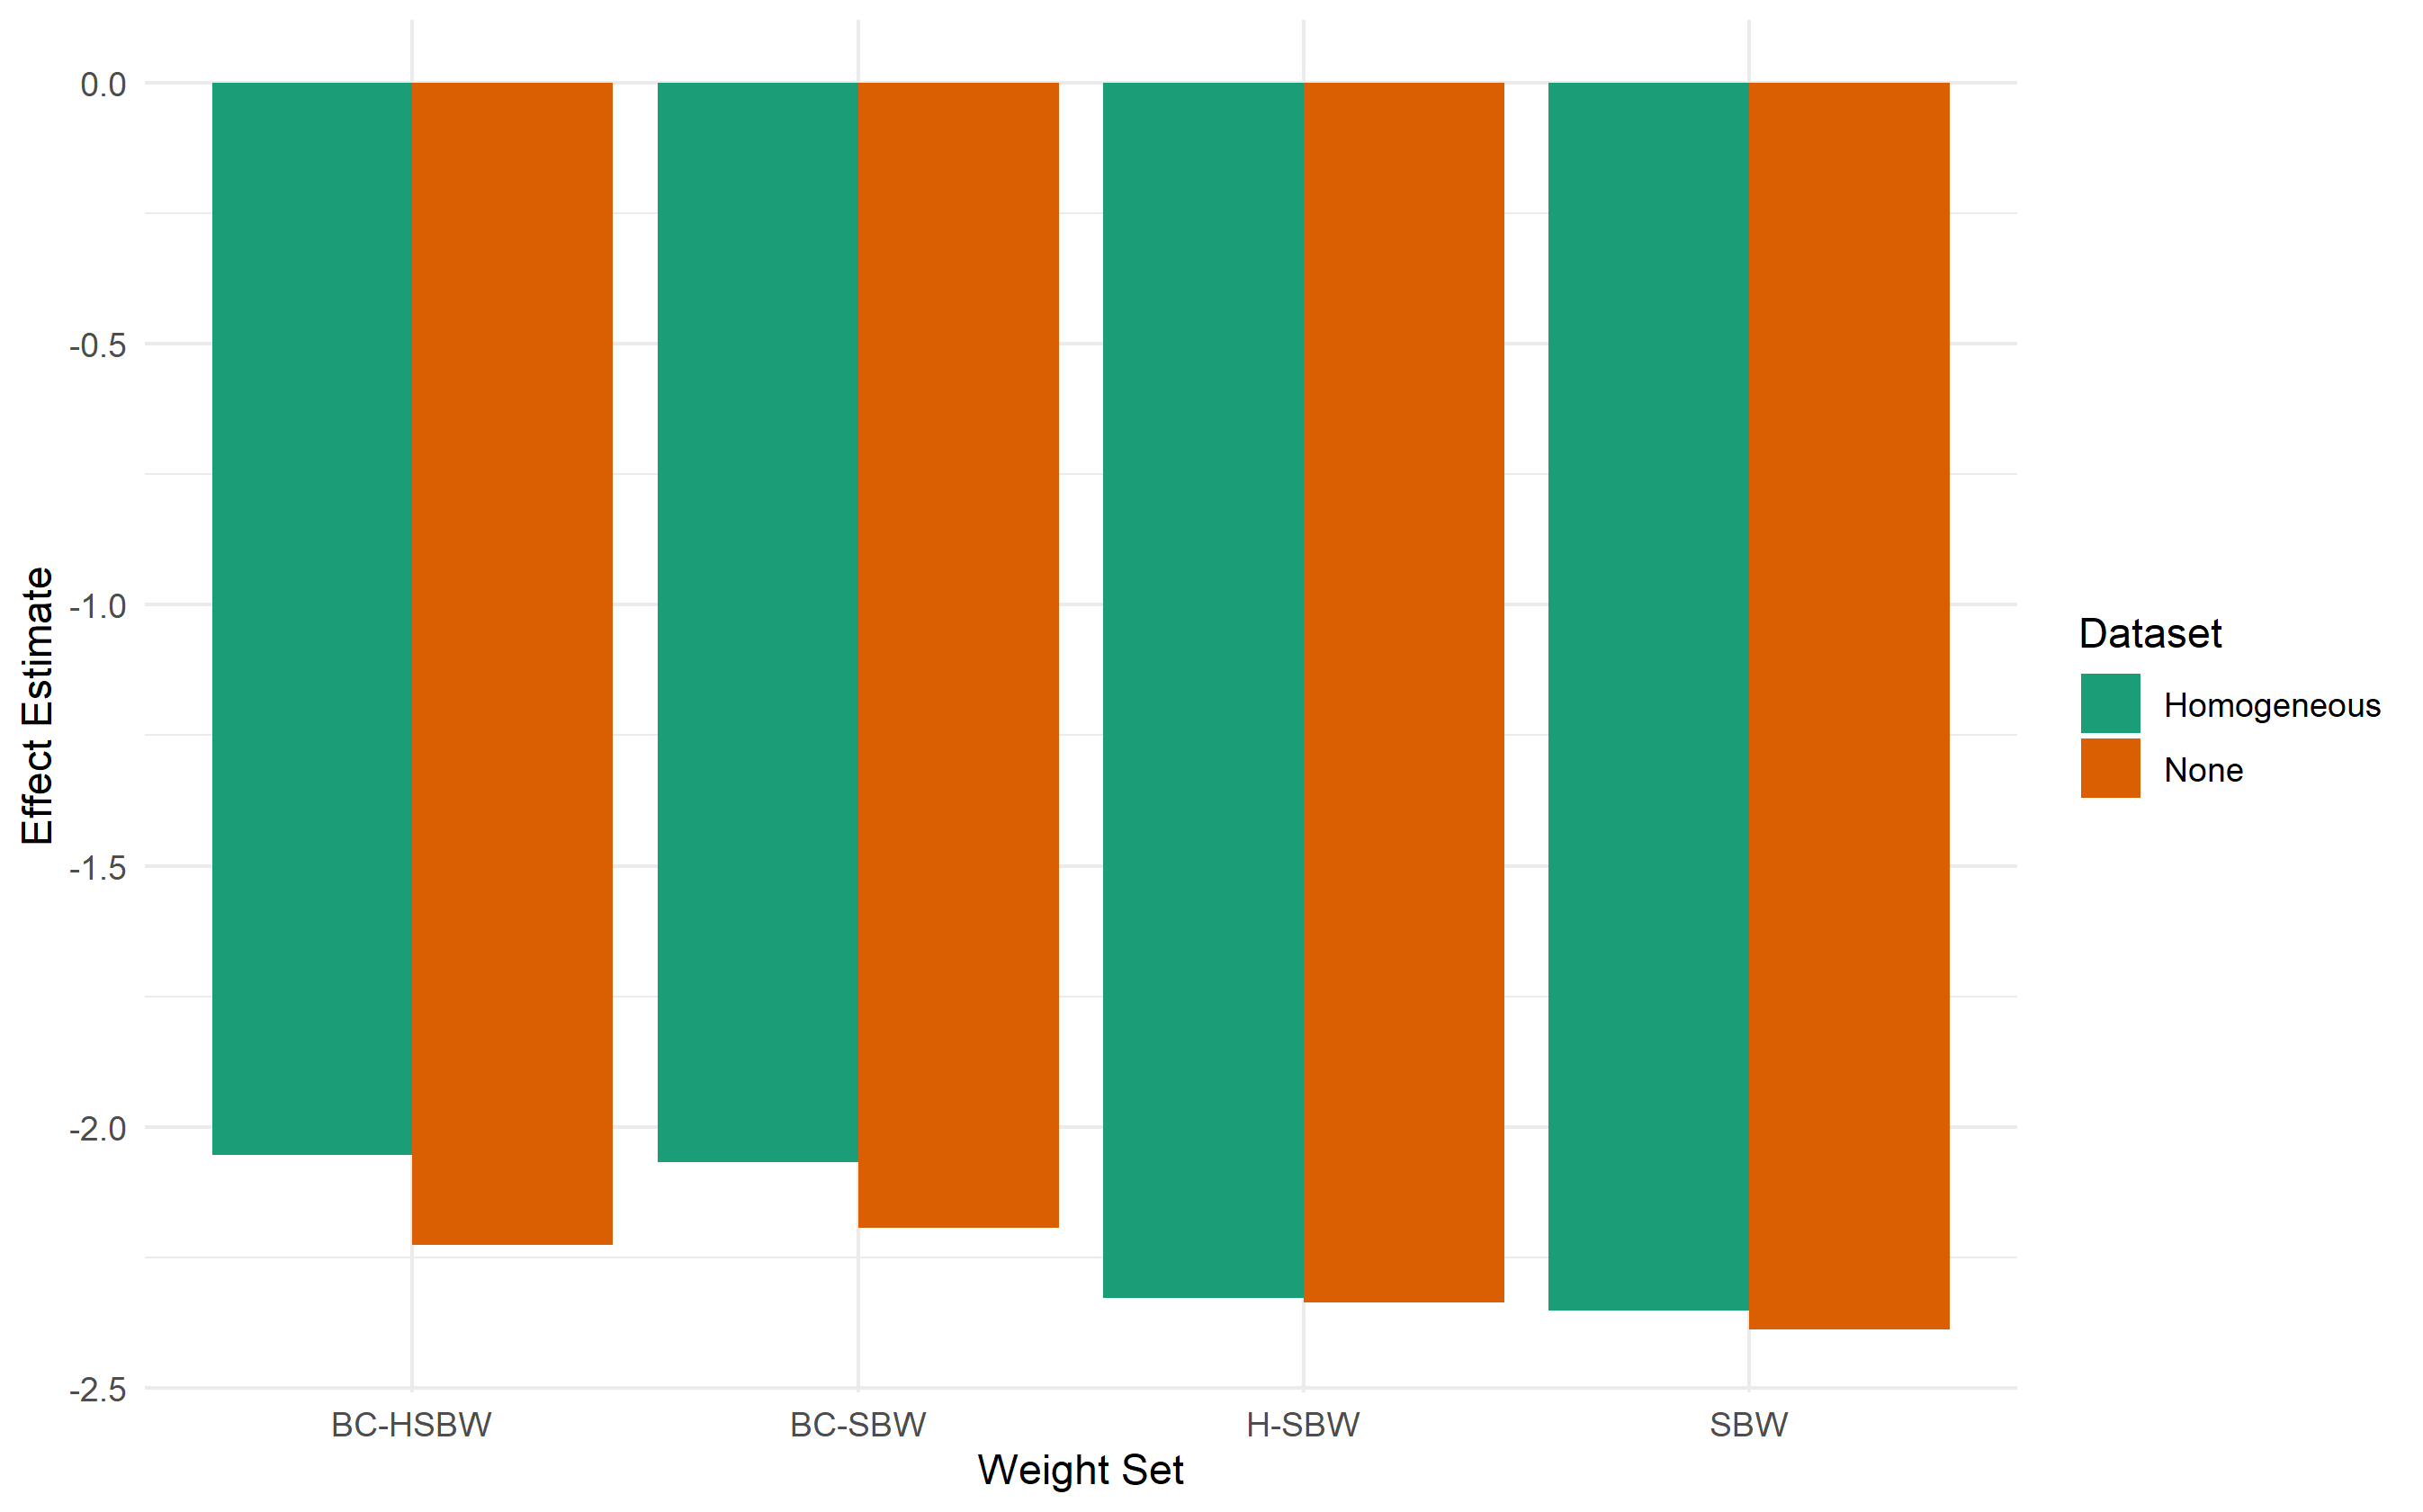
\includegraphics[scale=0.6]{01_Plots/point-estimates-c1.png}
\end{center}
\end{figure}

Lastly, we examine the robustness of our point estimates to the removal of individual states (these are the same point estimates used to calculate our confidence intervals). Figure~\ref{fig:loostateplot} shows how the point estimates for each estimator changes for both the (homogeneous) adjusted and unadjusted datasets. We see similar results in either case: removing Ohio tends to move the point estimates farther from zero (though the change is larger on the adjusted dataset). By contrast, removing North Dakota, Kentucky, or California tends to move the estimates closer to zero. 

\begin{figure}[H]
\begin{center}
    \caption{Estimator sensitivity to states}
    \label{fig:loostateplot}
    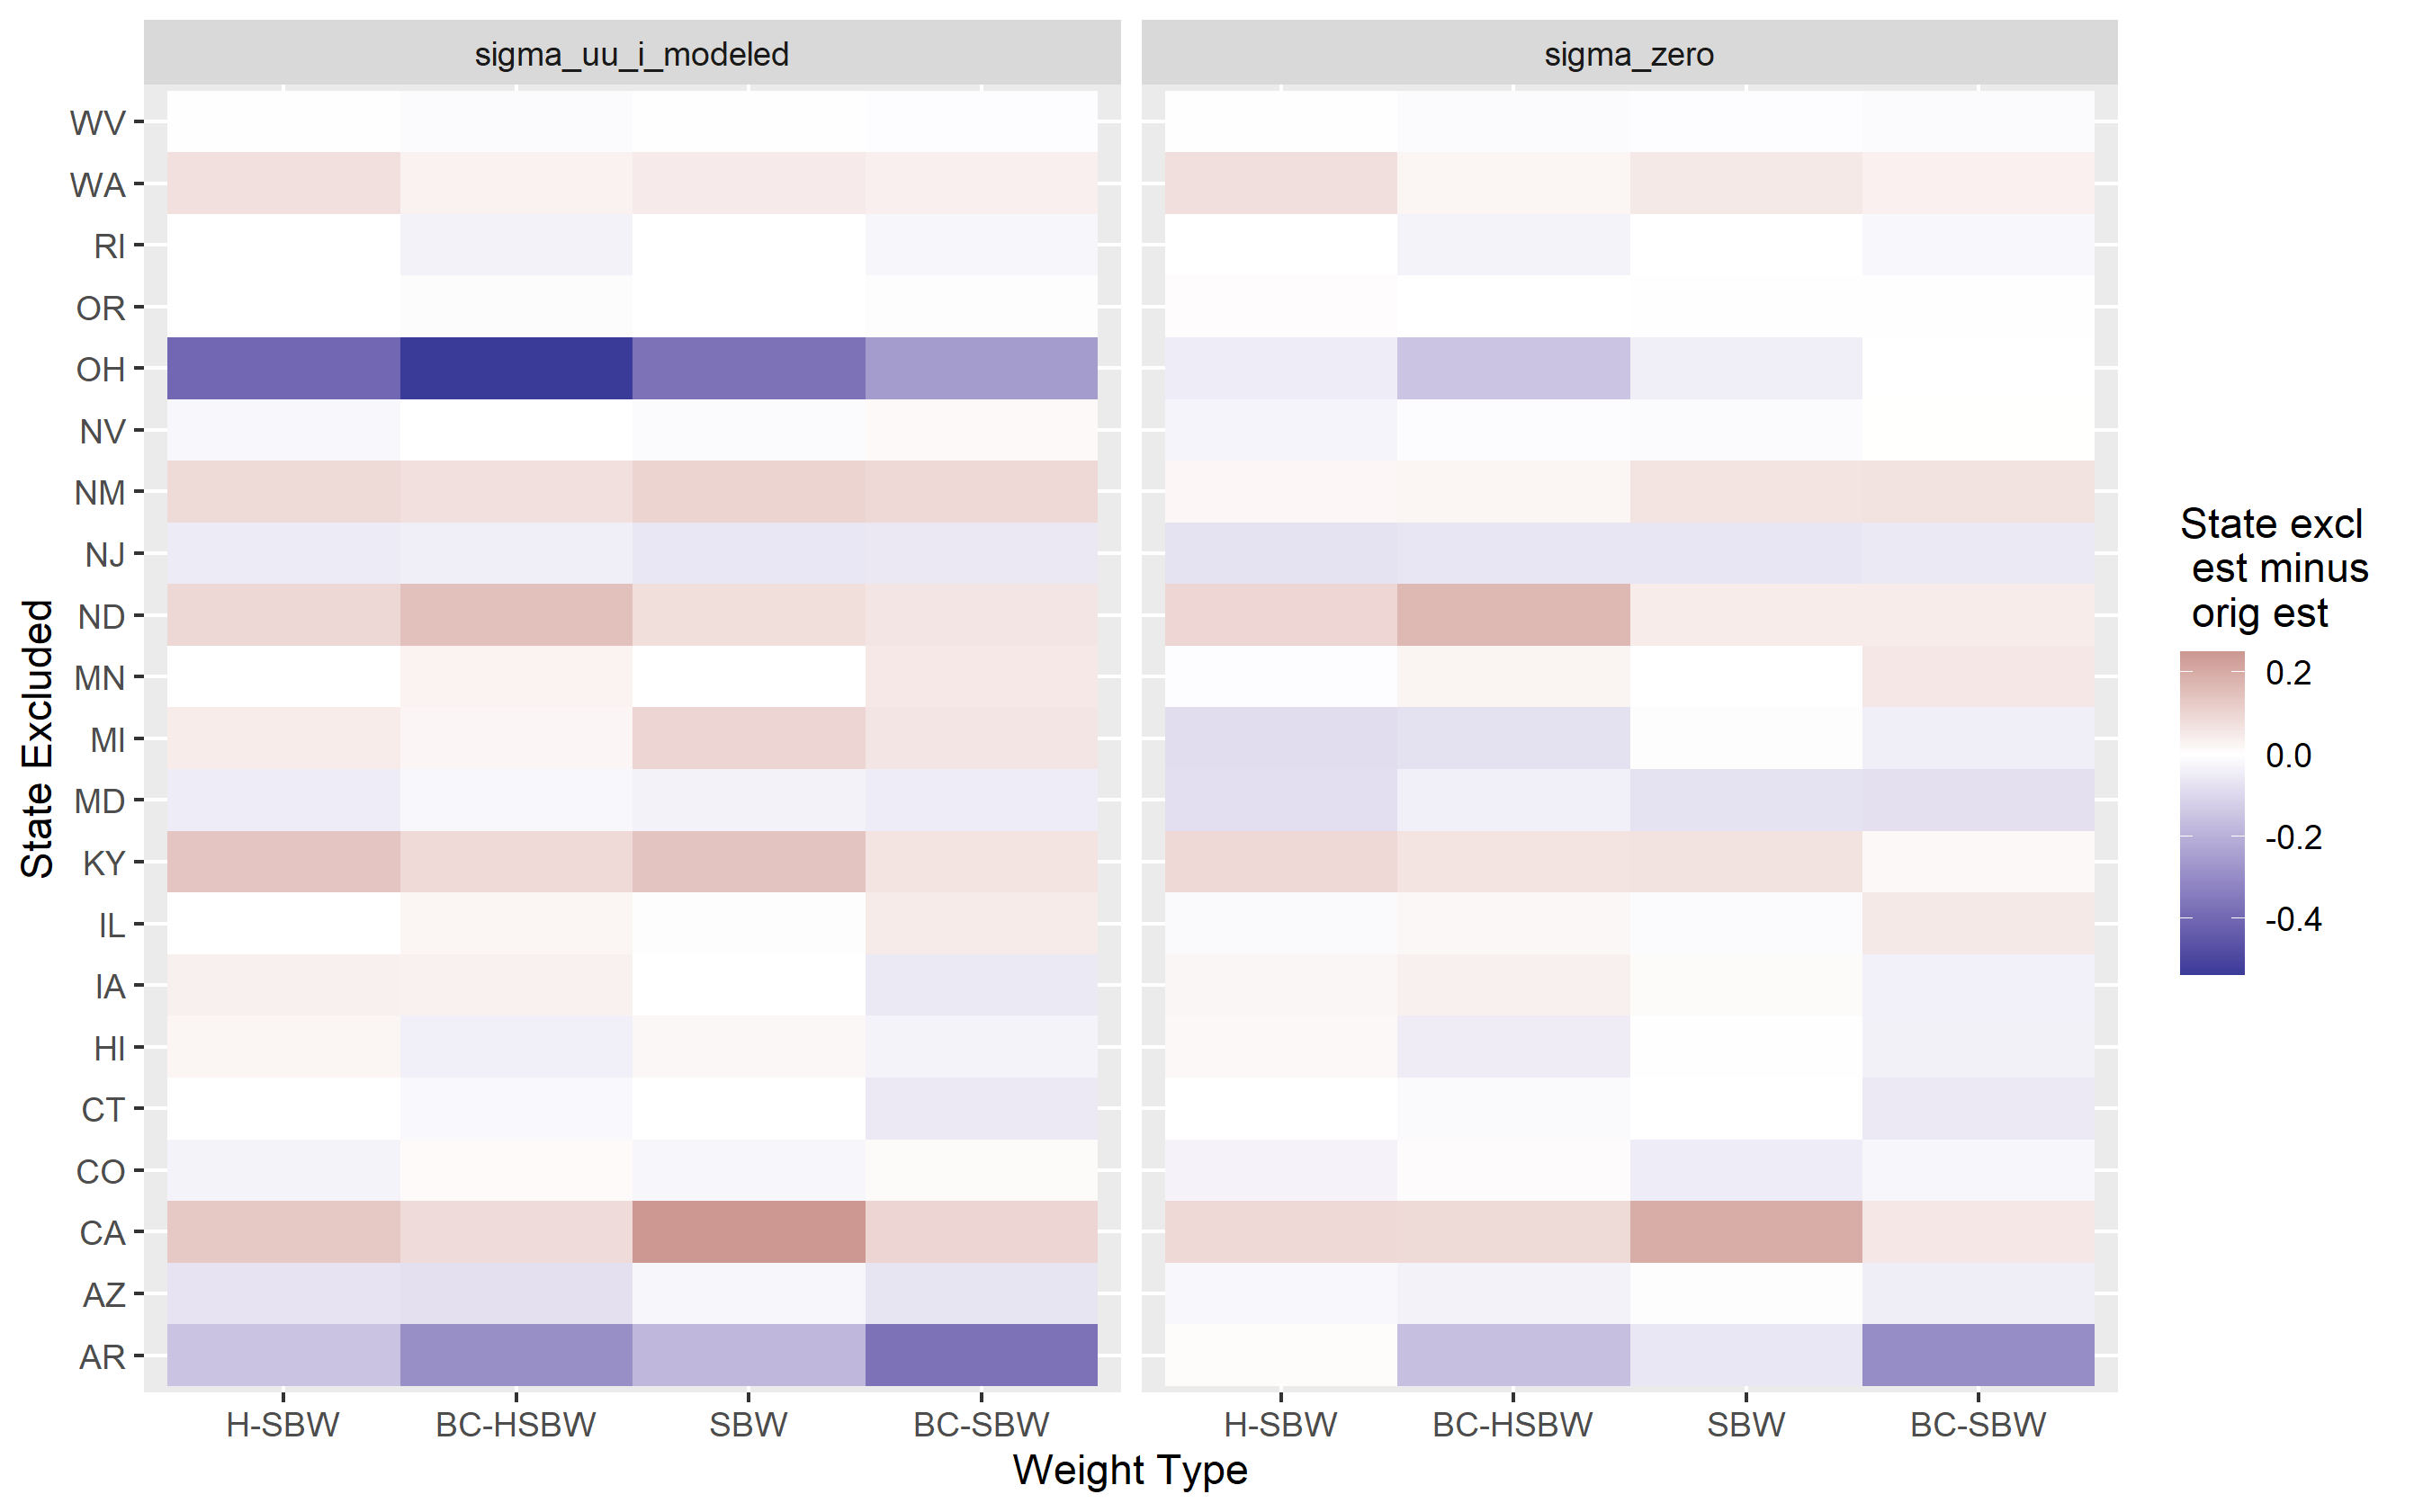
\includegraphics[scale=0.6]{01_Plots/loostate-sensitivityc1-state-uu-i.png}
\end{center}
\end{figure}

\subsection{Sensitivity analysis} \label{sssec:sensitivity}

We now consider the sensitivity of our analysis with respect to no anticipatory treatment effects. Several states had partial limited expansions prior to 2014. Following \cite{frean2017premium}, these states are California, Connecticut, Minnesota, New Jersey, and Washington. We rerun our analyses excluding CPUMAs from all five of these states. We have no a priori expectation about how removing these states might affect our estimates: on the one hand, states that expanded early might have a smaller treatment effect after 2014 because they already enrolled newly eligible individuals. On the other hand, if these states were also more motivated to enroll people in Medicaid, they might have experienced larger post-expansion coverage gains. Figure~\ref{fig:weightsbystatec2} in Appendix D displays the H-SBW weights summed by state alongside BC-HSBW, which extrapolates to reduce the imbalances. 

Excluding early expansion states, we estimate an effect of -2.09 (-2.85, -1.33) percentage points using H-SBW weights and -2.05 (-2.75, -1.35) percentage points for SBW. These estimates are quite similar to though slightly closer to zero than the the primary estimates. We also see that the differential between these estimates and the unadjusted estimates is slightly larger: -2.28  (-2.82, -1.74) percentage points for H-SBW and -2.21 (-2.71, -1.72) percentage points for SBW. 

When we add the bias-correction the point estimates again move closer to zero: -1.94 (-2.96, -0.92) percentage points for BC-HSBW and -1.99 (-3, -0.99) percentage points for BC-SBW. Overall these results suggests that the results are relatively robust to the exclusion of these states, so that potential violations of this causal assumption do not appear to be a large factor.

\subsection{Covariate importance}

We also investigate our hypothesis that factors associated with Governance are associated with treatment response. As discussed above, we first remove the balance constraints on the Republican governance indicators and estimate $\hat{\psi}^1_v$, and then subtract our original ETC point estimate from this quantity to generate $\hat{\Delta}_v^1$. Because this quantity does not reflect a clear population target, instead of confidence intervals, we present the minimum and maximum leave-one-state-out values in parentheses next to the original estimate.

For the H-SBW estimator we calculate $\hat{\Delta}^1$ equal to -0.69 (min = -0.83, max = -0.42) and equal to -0.79 (min = -0.90, max = -0.66) on our unadjusted dataset. In other words, our primary estimated treatment effect moved 0.78 percentage points further away from zero when we excluded the Republican governance indicators. This reflects a 33 percent decrease in our point estimate, a not-unsubstantial difference. Moreover, all of these estimates were less than zero, regardless of whether we conditioned on the covariate adjustment or not, regardless of whether we remove the early expansion states or not, and when removing each state. Across all specifications that we ran the minimum change we calculated was -1.34 and the maximum was -0.36. Additional distributional results across all leave-one-state-out estimates are available in Appendix E, Table~\ref{tab:rdiffc1}. Figure~\ref{fig:repub} displays our estimates of $\hat{\Delta}_v^1$ on our primary dataset and removing early expansion states (conditional on the covariate adjustment). 

We also consider four other covariate sets. We find that our estimates are most sensitive to controlling for pre-treatment outcomes and unemployment rates. This is not unexpected: all else equal, the expansion region had much lower pre-treatment uninsurance rates. If we do not control for these covariates, the comparable region will likely have lower pre-treament uninsurance rates, causing the estimated counterfactual to be closer to zero. The effect estimates were less sensitive to the removal of other covariate groups, and all point estimates are available in Appendix E, Table~\ref{tab:ptests}.

\begin{figure}[H]
\begin{center}
    \caption{Removing Republican Governance Indicators}
    \label{fig:repub}
    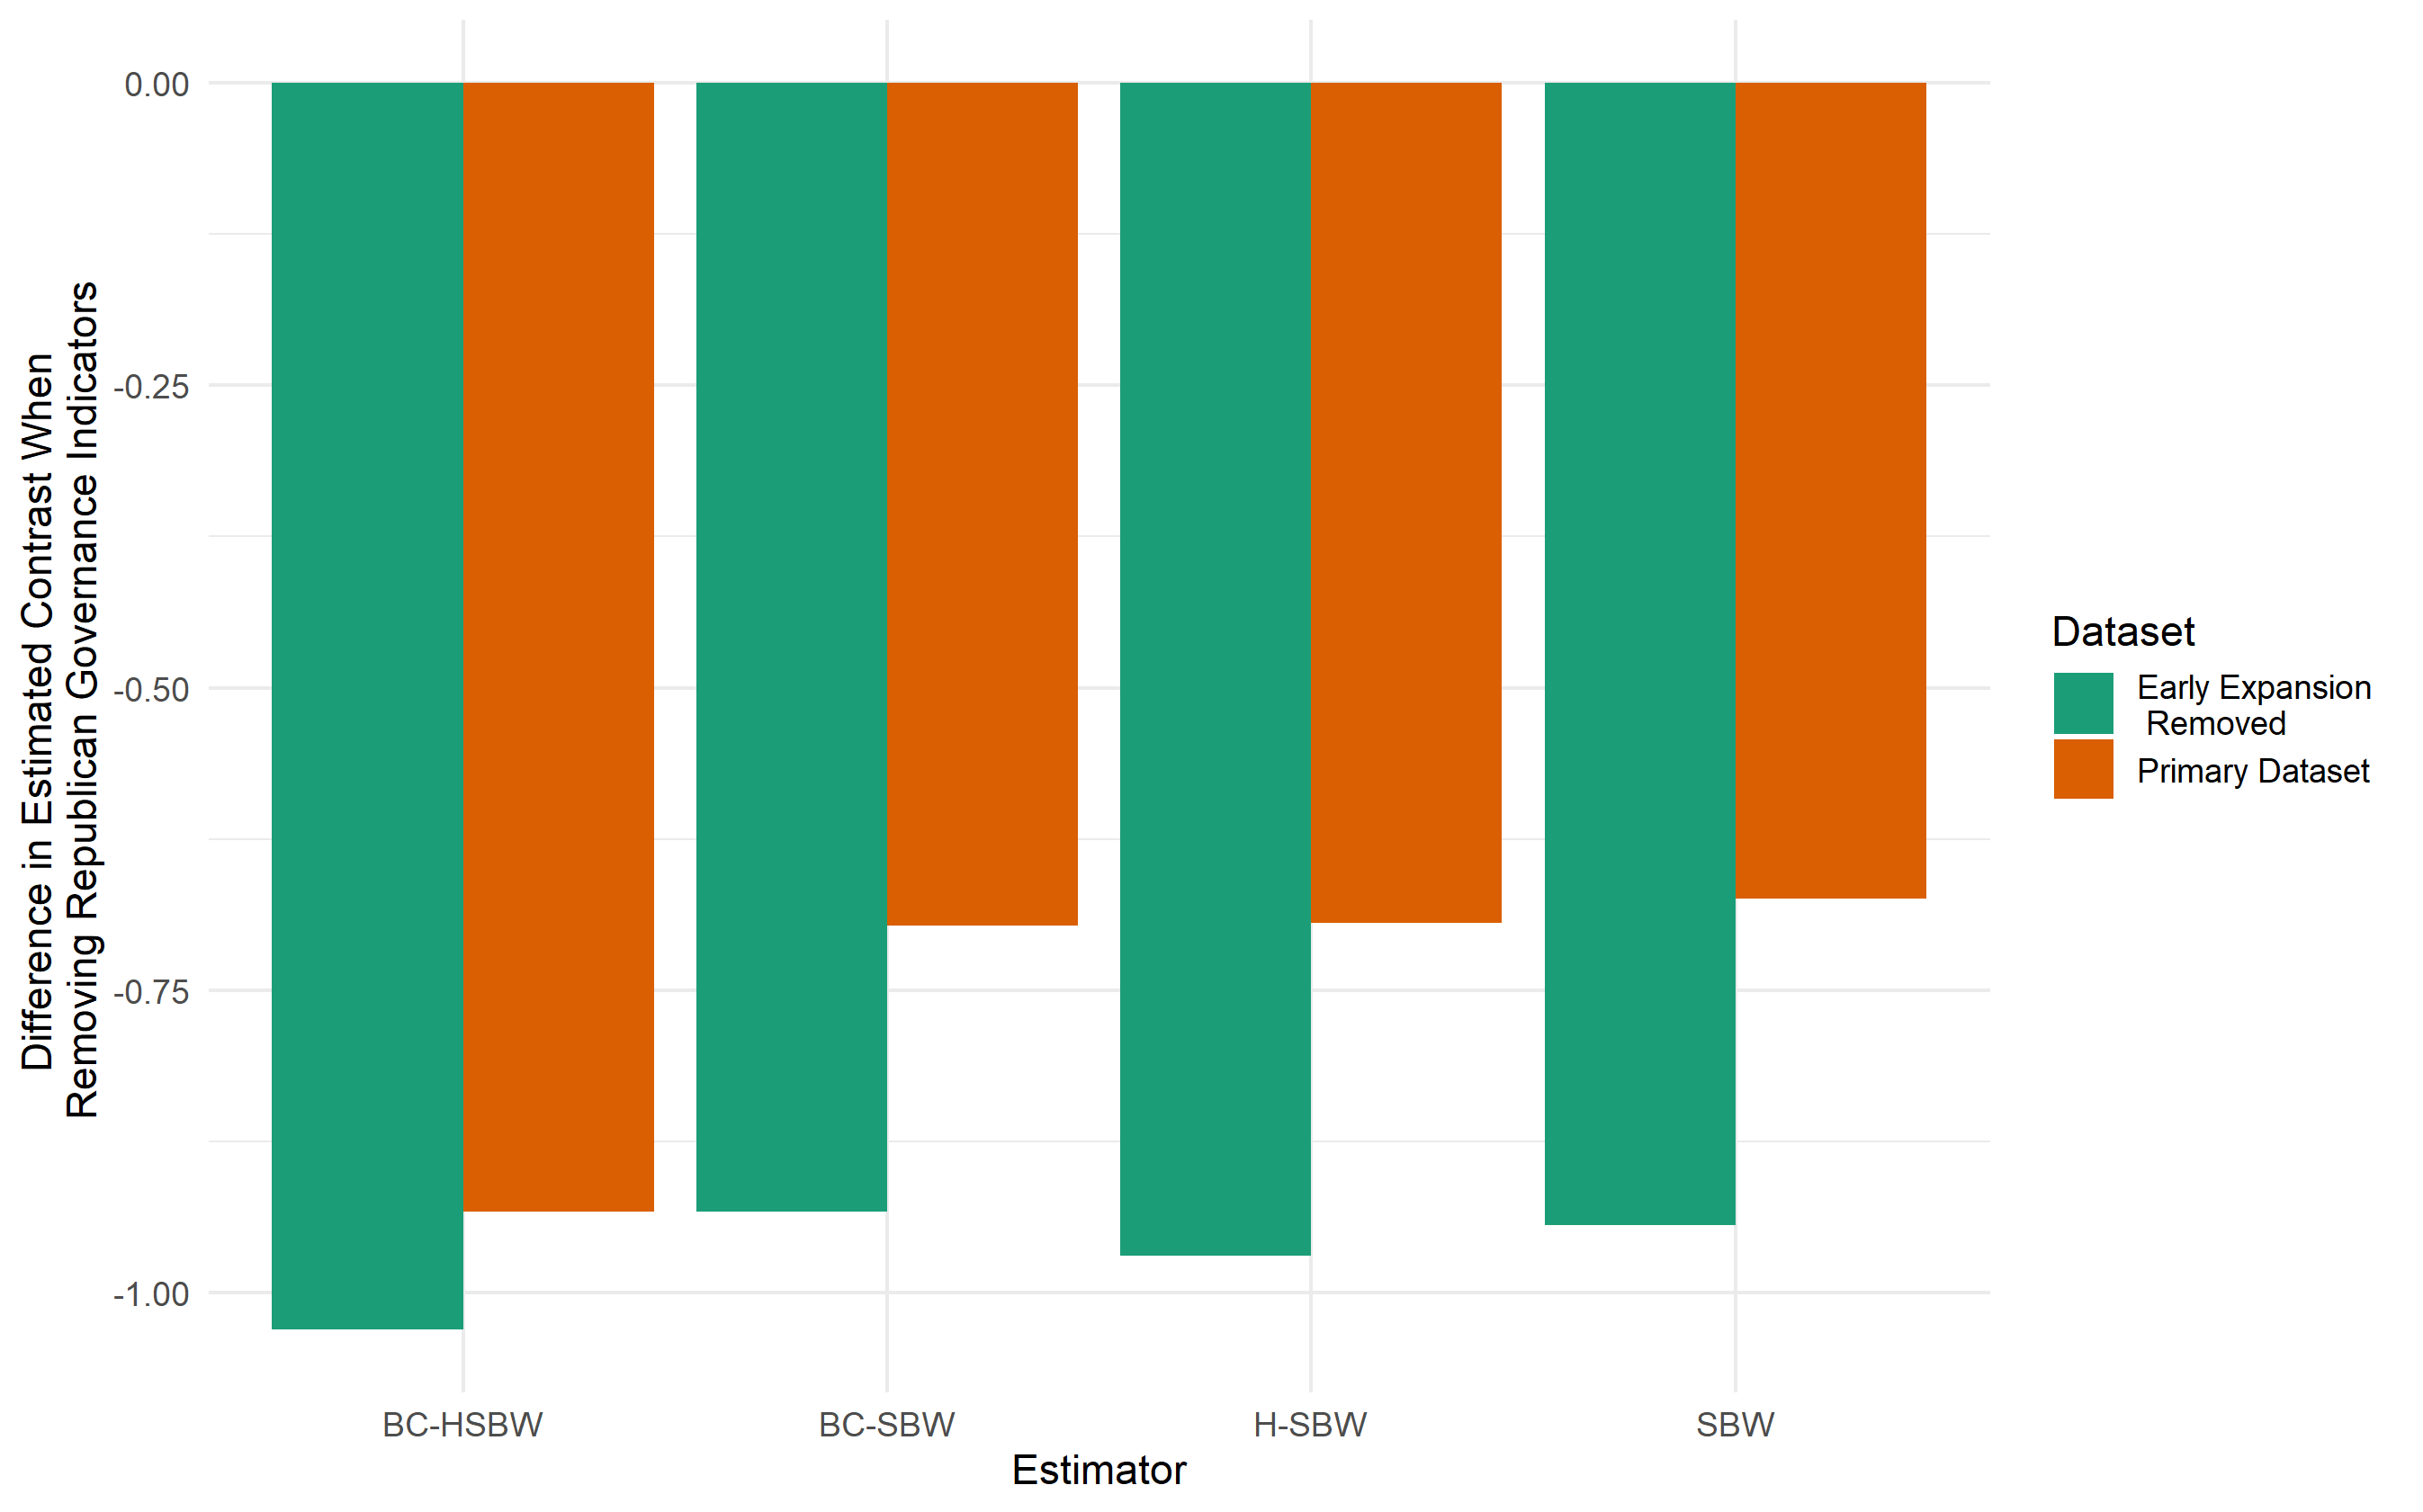
\includegraphics[scale=0.6]{01_Plots/repub-diff-all-estimators.png}
\end{center}
\end{figure}

These results highlight the importance of Republican governance in our counterfactual outcome model of $Y^1$. If the models specified by \cite{kaestner2017effects} and \cite{courtemanche2017early} are correct (that is, they correctly omit Republican governance from their balancing weights for estimating $Y^0$), this would suggest treatment effect heterogeneity with respect to Republican governance. Moreover, because the expansion-state region is much more Democratic than the non-expansion region, this heterogeneity could potentially drive differences between the ETC and the ETT.

Since this is a policy question of some interest, we directly investigate this by estimating the outcome model on the full data with treatment assignment interacted with each covariate \footnote{For this analysis we calculate separate covariate adjustments on the untreated data. The summary statistics for this adjustment are available in Appendix D.}. We then examine how the estimated treatment effect would change if we decreased the interaction between treatment assignment and each Republican governance indicator -- Republican governor, Republican lower legislature control, and Republican total control -- by 50 percentage points (note that the original variables are either 0 or 100 and measured at the state level). This linear combination of coefficients estimates how the treatment effect would change for any given collection of states against a set that is identical except for being 50 percentage points lower, on average, across the Republican governance indicators. We find that the linear combination is positive (0.21 percentage points) and statistically significant on the unadjusted dataset. This would indicate that the estimated treatment effect may be larger among Republican governed areas. However, this finding is not robust to any other specification that we run. Ultimately we interpret these results as providing no evidence of treatment effect heterogeneity with respect to Republican governance (though this analysis does not rule out this possibility either). The full results are available in Appendix E, Table~\ref{tab:hte}.